%!TEX encoding = UTF-8 Unicode
%!TEX root = ../lect-week03.tex


\Subsection{Funktioner}



\begin{Slide}{Deklarera funktioner, överlagring}
\begin{itemize}
\item En parameter, och sedan två parametrar:
\begin{REPL}
scala> :paste
  def öka(a: Int): Int = a + 1
  def öka(a: Int, b: Int) = a + b
  
scala> öka(1)
res0: Int = 2

scala> öka(1,1)
res1: Int = 2

\end{REPL}
\item Båda funktionerna ovan kan finnas samtidigt! Trots att de har samma namn är de \Alert{olika} funktioner; kompilatorn kan skilja dem åt med hjälp av de olika parameterlistorna.

\item Detta kallas \Emph{överlagring} \Eng{overloading} av funktioner.

\end{itemize}
\end{Slide} 


\begin{Slide}{Tom parameterlista och inga parametrar}\SlideFontSmall
\begin{itemize}
\item Om en funktion deklareras med tom parameterlista \code{()} kan den anropas på två sätt: med och utan tomma parenteser.
\begin{REPL}
scala> def tomParameterLista() = 42

scala> tomParameterLista()
res2: Int = 42

scala> tomParameterLista
res3: Int = 42
\end{REPL}

Denna flexibilitet är grunden för \Emph{enhetlig access}: namnet kan användas enhetligt oavsett om det är en funktion eller en variabel.
\item Om parameterlista saknas får man \Alert{inte} använda \code{()} vid anrop:

\begin{REPL}
scala> def ingenParameterLista = 42

scala> ingenParameterLista
res4: Int = 42

scala> ingenParameterLista()
<console>:13: error: Int does not take parameters
       ingenParameterLista()
\end{REPL}

\end{itemize}
\end{Slide} 


\begin{Slide}{Funktioner med defaultargument}\SlideFontSmall

\begin{itemize}
\item Vi kan ofta åstadkomma något som liknar överlagring, men med en enda funktion, om vi i stället använder \Emph{defaultargument}:
\begin{REPLnonum}
scala> def inc(a: Int, b: Int = 1) = a + b
inc: (a: Int, b: Int)Int

scala> inc(42, 2)
res0: Int = 44

scala> inc(42, 1)
res1: Int = 43

scala> inc(42)
res2: Int = 43

\end{REPLnonum}
\item Om argumentet utelämnas och det finns ett defaultargumentet, så är det defaultargumentet som appliceras.
\end{itemize}
\end{Slide} 


\begin{Slide}{Funktioner med namngivna argument}
\begin{itemize}
\item Genom att använda \Emph{namngivna argument} behöver man inte hålla reda på ordningen på parametrarna, bara man känner till parameternamnen. 
\item Namngivna argument går fint att \Alert{kombinera} med defaultargument.
\begin{REPL}
scala> def namn(förnamn: String, 
                efternamn: String, 
                förnamnFörst: Boolean = true,
                ledtext: String = ""): String = 
         if (förnamnFörst) s"$ledtext: $förnamn $efternamn" 
         else s"$ledtext: $efternamn, $förnamn"

scala> namn(ledtext = "Name", efternamn = "Coder", förnamn = "Kim")
res0: String = Name: Kim Coder
\end{REPL}
\end{itemize}
\end{Slide} 


\begin{Slide}{Anropsstacken och objektheapen}\SlideFontSmall
Minnet är uppdelat i två delar:
\begin{itemize}
\item \Emph{Anropsstacken}: På stackminnet läggs en \Emph{aktiveringspost} \Eng{stack frame\footnote{\href{https://en.wikipedia.org/wiki/Call_stack}{en.wikipedia.org/wiki/Call\_stack}}, activation record} för varje funktionsanrop med plats för parametrar och lokala variabler. Aktiveringsposten raderas när returvärdet har levererats. Stacken växer vid nästlade funktionsanrop, då en funktion i sin tur anropar en annan funktion. 

\item \Emph{Objektheapen}: I heapminnet\footnote{\href{https://en.wikipedia.org/wiki/Memory_management}{en.wikipedia.org/wiki/Memory\_management}}$^{,}$\footnote{Ej att förväxlas med datastrukturen heap  \href{https://sv.wikipedia.org/wiki/Heap}{sv.wikipedia.org/wiki/Heap}} sparas alla objekt (data) som allokeras under körning. Heapen städas vid tillfälle av skräpsamlaren \Eng{garbage collector}, och minne som inte används längre frigörs. \\\vspace{0.5em}
\href{http://stackoverflow.com/questions/1565388/increase-heap-size-in-java}{stackoverflow.com/questions/1565388/increase-heap-size-in-java}
\end{itemize}
\end{Slide} 


\begin{Slide}{Aktiveringspost}\SlideFontSmall
Nästlade anrop ger växande anropsstack.
\begin{REPL}
scala> :paste
def f(): Unit = { val n = 5; g(n, 2 * n) }
def g(a: Int, b: Int): Unit = { val x = 1; h(x + 1, a + b) }
def h(x: Int, y: Int): Unit = { val z = x + y; println(z) }

scala> f()

\end{REPL}

\pause
\Alert{Stacken}

\begin{tabular}{|r | l | l |} \hline

variabel & värde & Vilken aktiveringspost? \\ \hline \hline
\pause
 n & 5 & f \\ \hline
 \pause 
 a & 5 & g \\
 b & 10 &  \\
 x & 1  &  \\  \hline
 \pause 
 x & 2  & h \\
 y & 15 &  \\
 z & 17 & \\ \hline
\end{tabular}
\end{Slide} 


\begin{Slide}{Lokala funktioner}\SlideFontSmall
Med lokala funktioner kan delproblem lösas med nästlade abstraktioner. 

\begin{Code}
def gissaTalet(max: Int): Unit = {
  def gissat = io.StdIn.readLine(s"Gissa talet mellan [1, $max]: ").toInt 
  val hemlis = (math.random * max + 1).toInt
  def skrivLedtrådOmEjRätt(gissning: Int): Unit = 
    if (gissning > hemlis) println(s"$gissning är för stort :(") 
    else if (gissning < hemlis) println(s"$gissning är för litet :(")
  def inteRätt(gissning: Int): Boolean = { 
    skrivLedtrådOmEjRätt(gissning)
    gissning != hemlis
  }
  def loop: Int = { var i = 1; while(inteRätt(gissat)){ i += 1 }; i }
  
  println(s"Du hittade talet $hemlis på $loop gissningar :)")
}
\end{Code}

Lokala, nästlade funktionsdeklarationer är tyvärr inte tillåtna i Java.\footnote{\href{http://stackoverflow.com/questions/5388584/does-java-support-inner-local-sub-methods}{\SlideFontSize{8}{9}stackoverflow.com/questions/5388584/does-java-support-inner-local-sub-methods}} 

\end{Slide} 



\begin{Slide}{Värdeanrop och namnanrop}\SlideFontSmall
\begin{itemize}
\item Det vi sett hittills är \Emph{värdeanrop}: argumentet evalueras \Alert{först} innan dess \Alert{värde} \emph{sedan} appliceras:
\begin{REPL}
scala> def byValue(n: Int): Unit = for (i <- 1 to n) print(" " + n)

scala> byValue(21 + 21)
 42 42 42 42 42 42 42 42 42 42 42 42 42 42 42 42 42 42 42 42 42 42 42 42 42 42 42 42 42 42 42 42 42 42 42 42 42 42 42 42 42 42

scala> byValue({print(" hej"); 21 + 21})
 hej 42 42 42 42 42 42 42 42 42 42 42 42 42 42 42 42 42 42 42 42 42 42 42 42 42 42 42 42 42 42 42 42 42 42 42 42 42 42 42 42 42 42
\end{REPL}
\item Men man kan med \code{=>} före parametertypen åstadkomma \Emph{namnanrop}: argumentet \Alert{''klistras in''} i stället för \Alert{namnet} och evalueras \Alert{varje gång} (kallas även \Emph{fördröjd evaluering}):
\begin{REPL}
scala> def byName(n: => Int): Unit = for (i <- 1 to n) print(" " + n)

scala> byName({print(" hej"); 21 + 21})
 hej hej 42 hej 42 hej 42 hej 42 hej 42 hej 42 hej 42 hej 42 hej 42 hej 42 hej 42 hej 42 hej 42 hej 42 hej 42 hej 42 hej 42 hej 42 hej 42 hej 42 hej 42 hej 42 hej 42 hej 42 hej 42 hej 42 hej 42 hej 42 hej 42 hej 42 hej 42 hej 42 hej 42 hej 42 hej 42 hej 42 hej 42 hej 42 hej 42 hej 42 hej 42 hej 42
\end{REPL}

\end{itemize}
\end{Slide} 

\begin{Slide}{Klammerparenteser vid ensam parameter}
Så här har vi sett nyss att man man göra:
\begin{REPL}
scala> def loop(n: => Int): Unit = for (i <- 1 to n) print(" " + n)

scala> loop(21 + 21)

scala> loop({print(" hej"); 21 + 21})
\end{REPL}

Men...\\För alla funktioner \code{f} gäller att: \\ det är helt ok att byta ut vanliga parenteser: \hfill\code{f(uttryck)} \\ mot krullparenteser: \hfill\code|f{uttryck}| \\ \Alert{om} parameterlistan har \Alert{exakt en} parameter.  

\vspace{0.5em}Men man kan alltså göra så här också:
\begin{REPLnonum}
scala> loop{ 21 + 21 }

scala> loop{ print(" hej"); 21 + 21 }
\end{REPLnonum}


\end{Slide} 

\begin{Slide}{Uppdelad parameterlista}
\begin{itemize}
\item Vi har tidigare sett att man kan ha mer än en parameter:
\begin{REPLnonum}
scala> def add(a: Int, b: Int) = a + b

scala> add(21, 21)
res0: Int = 42
\end{REPLnonum}

\item Man kan även ha \Alert{mer än en} parameterlista:
\begin{REPLnonum}

scala> def add(a: Int)(b: Int) = a + b

scala> add(21)(21)
res1: Int = 42
\end{REPLnonum}
\item Detta kallas även \Emph{multipla parameterlistor} \Eng{multiple parameter lists}
\end{itemize}
\href{http://docs.scala-lang.org/style/declarations.html#multiple-parameter-lists}{\SlideFontTiny docs.scala-lang.org/style/declarations.html\#multiple-parameter-lists}
\end{Slide} 


\begin{Slide}{Skapa din egen kontrollstruktur}
\begin{itemize}
\item Genom att \Alert{kombinera} \Emph{uppdelad parameterlista} med \Emph{namnanrop} med \Emph{klammerparentes vid ensam parameter} kan vi skapa vår egen kontrollstruktur:
\begin{REPLnonum}
scala> def upprepa(n: Int)(block: => Unit) = { 
         var i = 0
         while (i < n) { block; i += 1 }
       }

scala> upprepa(42){ 
         if (math.random < 0.5) {
           print(" gurka")
         } else {
           print(" tomat")
         }
       }
 gurka gurka gurka tomat tomat gurka gurka gurka gurka tomat tomat tomat tomat tomat gurka tomat tomat tomat tomat tomat tomat tomat tomat tomat gurka gurka gurka tomat tomat gurka gurka gurka tomat tomat gurka tomat gurka gurka gurka gurka tomat tomat
\end{REPLnonum}
\end{itemize}
\end{Slide} 


\begin{Slide}{Funktioner är äkta värden i Scala}\SlideFontSmall
\begin{itemize}
\item En funktioner är ett äkta värde.
\item Vi kan till exempel tilldela en variabel ett funktionsvärde. 
\item Med hjälp av blank+understreck efter funktionsnamnet får vi funktionen som ett \Alert{värde} (inga argument appliceras än):
\begin{REPLnonum}
scala> def add(a: Int, b: Int) = a + b

scala> val f = add _

scala> f
f: (Int, Int) => Int = <function2>

scala> f(21, 21)
res0: Int = 42
\end{REPLnonum}

\item Ett funktionsvärde har en \Alert{typ} precis som alla värden: \\ 
\code{f: (Int, Int) => Int}
\end{itemize}
\end{Slide} 

\begin{Slide}{Funktionsvärden kan vara argument}
\begin{itemize}
\item En funktion kan ha en annan funktion som parameter:
\begin{REPL}
scala> def tvåGånger(x: Int, f: Int => Int) = f(f(x))

scala> def öka(x: Int) = x + 1

scala> def minska(x: Int) = x - 1

scala> tvåGånger(42, öka _)
res1: Int = 43

scala> tvåGånger(42, minska _)
res1: Int = 41
\end{REPL}

\item Om argumentets funktionstyp \Alert{kan härledas} av kompilatorn och \Alert{passar} med parametertypen så behövs ej understreck: \\ 
\begin{REPL}
scala> tvåGånger(42, öka)
res1: Int = 43
\end{REPL}\end{itemize}
\end{Slide}



\begin{Slide}{Applicera funktioner på element i samlingar med \texttt{map}}\SlideFontSmall
\begin{REPL}
scala> def öka(x: Int) = x + 1

scala> def minska(x: Int) = x - 1

scala> val xs = Vector(1, 2, 3)

scala> xs.map(öka)
res0: scala.collection.immutable.Vector[Int] = Vector(2, 3, 4)

scala> xs.map(minska)
res1: scala.collection.immutable.Vector[Int] = Vector(0, 1, 2)

scala> xs map öka
res2: scala.collection.immutable.Vector[Int] = Vector(2, 3, 4)

scala> xs map minska
res3: scala.collection.immutable.Vector[Int] = Vector(0, 1, 2)
\end{REPL}
Funktioner som tar andra funktioner som parametrar kallas \\ \Emph{högre ordningens funktioner}. 
\end{Slide} 




\begin{Slide}{Anonyma funktioner}
\begin{itemize}
\item  Man behöver inte ge funktioner namn. De kan i stället skapas med hjälp av \Emph{funktionsliteraler}.\footnote{Även kallat ''lambda-värde'' eller bara ''lamda'' efter den s.k. lambdakalkylen. \href{https://en.wikipedia.org/wiki/Anonymous_function}{en.wikipedia.org/wiki/Anonymous\_function}}

\item En funktionsliteral har ...
\begin{enumerate}
\item en parameterlista (utan funktionsnamn) och ev. returtyp, \item sedan den reserverade teckenkombinationen \code{=>} \item och sedan ett uttryck (eller ett block).
\end{enumerate}
\item Exempel:
\begin{Code}[basicstyle=\ttfamily\fontsize{10}{12}\selectfont]
(x: Int, y: Int): Int => x + y
\end{Code}
\pause
\item Om kompilatorn kan gissa typerna från sammanhanget så behöver typerna inte anges i själva  funktionsliteralen:
\begin{Code}[basicstyle=\ttfamily\fontsize{10}{12}\selectfont]
val f: (Int, Int) => Int = (x, y) => x + y
\end{Code}

\end{itemize}
\end{Slide}


\begin{Slide}{Applicera anonyma funktioner på element i samlingar}\SlideFontSmall
\begin{itemize}
\item Anonym funktion skapad med funktionsliteral direkt i anropet:
\begin{REPL}
scala> val xs = Vector(1, 2, 3)

scala> xs.map((x: Int): Int => x + 1)
res0: scala.collection.immutable.Vector[Int] = Vector(2, 3, 4)
\end{REPL}
\item Eftersom kompilatorn här kan härleda typerna så behövs de inte:
\begin{REPL}
scala> xs.map(x => x - 1)
res1: scala.collection.immutable.Vector[Int] = Vector(0, 1, 2)

scala> xs map (x => x - 1)
res2: scala.collection.immutable.Vector[Int] = Vector(0, 1, 2)

\end{REPL}
\item Om man bara använder parametern en enda gång i funktionen så kan man byta ut parameternamnet mot ett understreck.

\begin{REPL}
scala> xs.map(_ + 1)
res3: scala.collection.immutable.Vector[Int] = Vector(2, 3, 4)
\end{REPL}
\end{itemize}
\end{Slide} 



\begin{Slide}{Platshållarsyntax för anonyma funktioner}\SlideFontSmall
\begin{itemize}
\item Understreck i funktionsliteraler kallas \Emph{platshållare} \Eng{placeholder} och medger ett förkortat skrivsätt \Alert{om} den parameter som understrecket representerar används \Alert{endast en gång}.

\begin{Code}[basicstyle=\ttfamily\fontsize{10}{12}\selectfont]
_ + 1
\end{Code}
Ovan expanderas av kompilatorn till följande funktionsliteral \\(där namnet på parametern är godtyckligt):
\begin{Code}[basicstyle=\ttfamily\fontsize{10}{12}\selectfont]
x => x + 1
\end{Code}
\pause
\item Det kan förekomma flera understreck; det första avser första parametern, det andra avser andra parametern etc.
\begin{Code}[basicstyle=\ttfamily\fontsize{10}{12}\selectfont]
_ + _
\end{Code}
... expanderas till:
\begin{Code}[basicstyle=\ttfamily\fontsize{10}{12}\selectfont]
(x, y) => x + y 
\end{Code}

\end{itemize}
\end{Slide} 


\begin{Slide}{Exempel på platshållarsyntax med samlingsmetoden \texttt{reduceLeft}}\SlideFontSmall
Metoden \code{reduceLeft} applerar en funktion på de två första elementen och tar sedan på resultatet som första argument och nästa element som andra argument och upprepar detta genom hela samlingen. 
\begin{REPL}
scala> def summa(x: Int, y: Int) = x + y

scala> val xs = Vector(1, 2, 3, 4, 5)

scala> xs.reduceLeft(summa)
res20: Int = 15

scala> xs.reduceLeft((x, y) => x + y)
res21: Int = 15

scala> xs.reduceLeft(_ + _)
res22: Int = 15

scala> xs.reduceLeft(_ * _)
res23: Int = 120
\end{REPL}
\end{Slide} 


\begin{Slide}{Stegade funktioner, ''Curry-funktioner''}
Om en funktion har en uppdelad parameterlista kan man skapa \Emph{stegade funktioner}, även kallat \Emph{partiellt applicerade} funktioner \Eng{partially applied functions} eller \Emph{''Curry''-funktioner}.
\begin{REPLnonum}
scala> def add(x: Int)(y: Int) = x + y  

scala> val öka = add(1) _
öka: Int => Int = <function1>

scala> Vector(1,2,3).map(öka)
res0:scala.collection.immutable.Vector[Int]= Vector(2, 3, 4)

scala> Vector(1,2,3).map(add(2))
res1:scala.collection.immutable.Vector[Int]= Vector(3, 4, 5)
\end{REPLnonum}
\end{Slide} 

\begin{Slide}{Översikt begrepp vi gått igenom hittills}
\begin{itemize}
\item överlagring
\item utelämna tom parameterlista (enhetlig access)
\item defaultargument
\item namngivna argument
\item lokala funktioner
\item namnanrop (fördröjd evaluering)
\item klammerparentes vid ensam paramenter
\item uppdelad parameterlista
\item egendefinierade kontrollstrukturer
\item funktioner som äkta värden
\item anonyma funktioner
\item stegade funktioner (''Curry-funktioner'')
\end{itemize}
\end{Slide} 

\begin{Slide}{Begränsningar i Java}\SlideFontTiny
\begin{itemize}
\item Av alla dessa funktionskoncept...
\begin{itemize}\SlideFontTiny
\item överlagring
\item utelämna tom parameterlista (principen om enhetlig access)
\item defaultargument
\item namngivna argument
\item lokala funktioner
\item namnanrop (fördröjd evaluering)
\item klammerparentes vid ensam paramenter
\item uppdelad parameterlista
\item egendefinierade kontrollstrukturer
\item funktioner som äkta värden
\item anonyma funktioner
\item stegade funktioner (''Curry-funktioner'')
\end{itemize}
\item ...kan man endast göra \Emph{överlagring} i Java 7, 
\item medan även \Emph{anonyma funktioner} (''lambda'') går att göra (med vissa begränsningar) i Java 8. \href{https://en.wikipedia.org/wiki/Anonymous_function\#Java_Limitations}{en.wikipedia.org/wiki/Anonymous\_function\#Java\_Limitations}
\item \vspace{0.5em} En av de saker jag saknar mest i Java: \Alert{lokala funktioner}!
\end{itemize}
Det är \Alert{kombinationen} av alla koncept som \Alert{skapar uttryckskraften} i Scala.

\end{Slide} 



\Subsection{Objekt}

\begin{Slide}{Objekt som modul}
\begin{itemize}
\item Ett \code{object} användas ofta för att samla \Emph{medlemmar} \Eng{members} som \Alert{hör ihop} och ge dem en egen \Emph{namnrymd} \Eng{name space}. 
\item Medlemmarna kan vara t.ex.: 
\begin{itemize}
\item  \code{val} \item \code{var} \item \code{def} 
\end{itemize}
\item Ett sådant objekt kallas även för \Emph{modul}.\footnote{
Även paket som skapas med \code{package} har en egen namnrymd och är därmed också en slags modul. Objekt kan alltså i Scala användas som ett alternativ till paket; en skillnad är att objekt kan ha tillstånd och att objekt inte skapar underkataloger vid kompilering (det finns iofs s.k. \code{package object}) \href{https://en.wikipedia.org/wiki/Modular_programming}{en.wikipedia.org/wiki/Modular\_programming}}

\end{itemize}

\end{Slide}

\begin{Slide}{Singelobjekt och metod} \SlideFontSmall
Ett Scala-\code{object} är ett s.k. \Emph{singelobjekt} \Eng{singleton object} och finns bara i \Alert{en} enda upplaga. \\ Minne för objektets variabler allokeras första gången objektet refereras. \\ En funktion som finns i ett objekt kallas en \Emph{metod} \Eng{method}.
\begin{Code}[basicstyle=\ttfamily\fontsize{9}{11}\selectfont]
object mittBankkonto {
  val kontonr: Long        = 1234567L
  var saldo: Int           = 1000
  def ärSkuldsatt: Boolean = saldo < 0
}
\end{Code}
\begin{REPLnonum}
scala> mittBankkonto.saldo -= 25000

scala> mittBankkonto.ärSkuldsatt
res0: Boolean = true
\end{REPLnonum}

(Vi ska i nästa vecka se hur man med s.k. klasser kan skapa många upplagor av samma  typ av objekt, så att vi kan ha flera olika bankkonto.)
\end{Slide} 



\begin{Slide}{Vad är ett tillstånd?} 
Ett objekts \Emph{tillstånd} är den samlade uppsättningen av värden av alla de variabler som finns i objektet.
\begin{Code}[basicstyle=\ttfamily\fontsize{9}{11}\selectfont]
object mittBankkonto {
  val kontonr: Long        = 1234567L
  var saldo: Int           = 1000
  def ärSkuldsatt: Boolean = saldo < 0
}
\end{Code}
\begin{tikzpicture}[font=\large\sffamily]
\matrix [matrix of nodes, row sep=0, column 2/.style={nodes={rectangle,draw,minimum width=0.8cm}}] (mat) 
{
\texttt{mittBankkonto}   &  \makebox(10,10){ }\\
%\texttt{g2}   &  \makebox(16,12){ }\\
};
\node[cloud, cloud puffs=13.0, cloud ignores aspect, minimum width=2cm, minimum height=3.8cm,
 align=center, draw] (x) at (5.8cm, -1.5cm) {
 \begin{tabular}{r l}
 \texttt{kontonr} & \fbox{1234567L} \\
 \texttt{saldo} & \fbox{1000}\\
 \end{tabular}
 };
\filldraw[black] (1.7cm,0.0cm) circle (3pt) node[] (ref) {};
 \draw [arrow, line width=0.7mm] (ref) -- (x);
% \node[cloud, cloud puffs=15.7, cloud ignores aspect, %minimum width=5cm, minimum height=2cm,
% align=center, draw] (g2) at (5cm, -2cm) {Gurka-\\objekt};
% \filldraw[black] (0.4cm,-0.4cm) circle (3pt) node[] (g2ref) {};
% \draw [arrow] (g2ref) -- (g2);
\end{tikzpicture}
\end{Slide} 


\begin{Slide}{Tillståndsändring} 

När en variabel tilldelas ett nytt värde sker en \Emph{tillståndsändring}. Ett \Emph{förändringsbart objekt} \Eng{mutable object} har ett \Emph{förändringsbart tillstånd} \Eng{mutable state}. 

\begin{REPLnonum}
scala> mittBankkonto.saldo -= 25000

scala> bankKonto.saldo
res1: Int = -24000
\end{REPLnonum}
\begin{tikzpicture}[font=\large\sffamily]
\matrix [matrix of nodes, row sep=0, column 2/.style={nodes={rectangle,draw,minimum width=0.8cm}}] (mat) 
{
\texttt{mittBankkonto}   &  \makebox(10,10){ }\\
%\texttt{g2}   &  \makebox(16,12){ }\\
};
\node[cloud, cloud puffs=13.0, cloud ignores aspect, minimum width=2cm, minimum height=3.8cm,
 align=center, draw] (x) at (5.8cm, -1.5cm) {
 \begin{tabular}{r l}
 \texttt{kontonr} & \fbox{1234567L} \\
 \texttt{saldo} & \fbox{-24000}\\
 \end{tabular}
 };
\filldraw[black] (1.7cm,0.0cm) circle (3pt) node[] (ref) {};
 \draw [arrow, line width=0.7mm] (ref) -- (x);
% \node[cloud, cloud puffs=15.7, cloud ignores aspect, %minimum width=5cm, minimum height=2cm,
% align=center, draw] (g2) at (5cm, -2cm) {Gurka-\\objekt};
% \filldraw[black] (0.4cm,-0.4cm) circle (3pt) node[] (g2ref) {};
% \draw [arrow] (g2ref) -- (g2);
\end{tikzpicture}
\end{Slide} 

\begin{Slide}{Vad rymmer sköldpaddan i Kojo i sitt tillstånd?} 
\begin{figure}
\centering
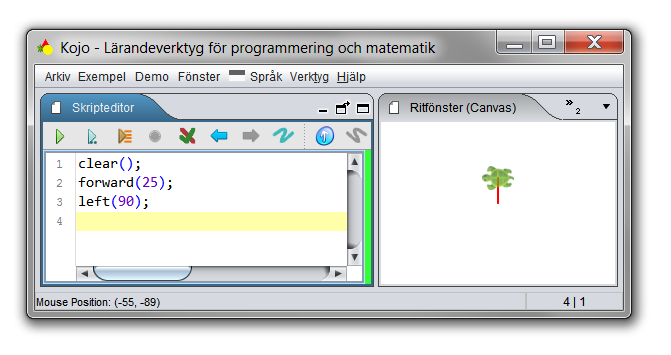
\includegraphics[width=0.7\textwidth]{../img/kojo}
\end{figure}
\pause position, rikting, pennfärg, pennbredd, penna uppe/nere, fyllfärg
\end{Slide} 

\begin{Slide}{Lata variabler och fördröjd evaluering} 
Med nyckelordet \code{lazy} före \code{val} skapas en s.k. ''lat'' \Eng{lazy} variabel.
\begin{REPL}
scala> val striktVektor = Vector.fill(1000000)(math.random)
striktVektor: scala.collection.immutable.Vector[Double] = 
 Vector(0.7583305221813246, 0.9016192590993339, 0.770022134260162, 0.15667718184929746, ...
 
scala> lazy val latVektor = Vector.fill(1000000)(math.random)
latVektor: scala.collection.immutable.Vector[Double] = <lazy>

scala> latVektor
res0: scala.collection.immutable.Vector[Double] = 
  Vector(0.5391685014341797, 0.14759775960530275, 0.722606095900537, 0.9025572787055386, ... 
\end{REPL}

En \code {lazy val} initialiseras \Alert{inte} vid deklarationen utan när den \Alert{refereras första gången}. Yttrycket som anges i deklarationen evalueras med s.k. \Emph{fördröjd evaluering} (även ''lat'' evaluering). 
\end{Slide} 

\begin{Slide}{Vad är egentligen skillnaden mellan \texttt{val}, \texttt{var}, \texttt{def} och \texttt{lazy val}?} 
\begin{Code}[basicstyle=\ttfamily\fontsize{8}{11}\selectfont]
object slump {
  val förAlltidSammaReferens  = math.random
  var kanÄndrasMedTilldelning = math.random
  def evaluerasVidVarjeAnrop  = math.random
  lazy val fördröjdInit       = Vector.fill(1000000)(math.random)
}
\end{Code}
\vspace{1em}\pause
Lat evaluering är en viktig princip inom funktionsprogrammering som möjliggör effektiva, oföränderliga datastrukturer där element allokeras först när de behövs. \\
\href{https://en.wikipedia.org/wiki/Lazy_evaluation}{en.wikipedia.org/wiki/Lazy\_evaluation}
\end{Slide} 


\Subsection{Funktioner är objekt}

\begin{Slide}{Programmeringsparadigm}
\href{https://en.wikipedia.org/wiki/Programming_paradigm}{en.wikipedia.org/wiki/Programming\_paradigm}:
\begin{itemize}
\item \Emph{Imperativ programmering}: programmet är uppbyggt av sekvenser av olika satser som läser och \Alert{ändrar} tillstånd
\item \Emph{Objektorienterad programmering}: en sorts imperativ programmering där programmet består av objekt som kapslar in tillstånd och erbjuder operationer som läser och \Alert{ändrar} tillstånd.
\item \Emph{Funktionsprogrammering}: programmet är uppbyggt av samverkande (matematiska) funktioner som \Alert{undviker} föränderlig data och tillståndsändringar. Oföränderliga datastrukturer skapar effektiva program i kombination med lat evaluering och rekursion. 
\end{itemize}
\end{Slide} 


\begin{Slide}{Funktioner är äkta objekt i Scala}
Scala visar hur man kan \Alert{förena} \Eng{unify} \\ \Emph{objekt-orientering} och \Emph{funktionsprogrammering}: \\\vspace{0.5em}

\textbf{\Large En funktion är ett objekt av funktionstyp\\ som har en \code{apply}-metod.}
\pause
\begin{REPLnonum}
scala> object öka extends (Int => Int) { 
         def apply(x: Int) = x + 1 
       }


scala> öka(1)
res0: Int = 2

scala> öka.   // tryck TAB
andThen   apply   compose   toString
\end{REPLnonum}
Mer om \code{extends} senare i kursen... %extends (Int => Int skrivs om till Function1[Int, Int]
\end{Slide} 


\Subsection{Rekursion}
\begin{Slide}{Rekursiva funktioner}
\begin{itemize}
\item Funktioner som \Alert{anropar sig själv} kallas \Emph{rekursiva}.


\begin{REPLnonum}
scala> def fakultet(n: Int): Int = 
         if (n < 2) 1 else n * fakultet(n - 1)

scala> fakultet(5)
res0: Int = 120
\end{REPLnonum}

\item För varje nytt anrop läggs en ny aktiveringspost på stacken. 

\item I aktiveringsposten sparas varje returvärde som gör att \code{5 * (4 * (3 * (2 * 1)))} kan beräknas. 

\item Rekrusionen avbryts när man når \Emph{basfallet}, här \code{n < 0}

\item En rekursiv funktion \Alert{måste} ha en returtyp.

\end{itemize}

\end{Slide} 

\begin{Slide}{Loopa med rekursion}
\begin{Code}
def gissaTalet(max: Int): Unit = {
  def gissat = io.StdIn.readLine(s"Gissa talet mellan [1, $max]: ").toInt 
  val hemlis = (math.random * max + 1).toInt
  def skrivLedtrådOmEjRätt(gissning: Int): Unit = 
    if (gissning > hemlis) println(s"$gissning är för stort :(") 
    else if (gissning < hemlis) println(s"$gissning är för litet :(")
  def ärRätt(gissning: Int): Boolean = { 
    skrivLedtrådOmEjRätt(gissning)
    gissning == hemlis
  }
  def loop(n: Int = 1): Int = if (ärRätt(gissat)) n else loop(n + 1)
  
  println(s"Du hittade talet $hemlis på ${loop()} gissningar :)")
}
\end{Code}
\end{Slide} 


\begin{Slide}{Rekursiva datastrukturer}

\begin{itemize}
\item Datastrukturena Lista och Träd är exempel på datastrukturer som passar bra ihop med rekursion. 
\item Båda dessa datastrukturer kan beskrivas rekursivt:
\begin{itemize}
\item En lista består av ett huvud och en lista, som i sin tur består av ett huvud och en lista, som i sin tur...
\item Ett träd består av grenar till träd som i sin tur består av grenar till träd som i sin tur, ...
\end{itemize}
\item Dessa datastrukturer bearbetas med fördel med rekursiva algoritmer.
\item I denna kursen ingår rekursion endast ''för kännedom'': \\ du ska veta vad det är och kunna skapa en enkel rekursiv funktion, t.ex. fakultets-beräkning. Du kommer jobba mer med rekursion och rekursiva datastrukturer i fortsättningskursen.
\end{itemize}
\end{Slide} 

\Subsection{SimpleWindow}
\begin{Slide}{Färdiga, enkla funktioner för att rita finns i klassen \texttt{cslib.window.SimpleWindow}}
På labben ska du använda \code{cslib.window.SimpleWindow}
\begin{itemize}
\item Paketet \code{cslib} innehåller paketet \code{window} som innehåller Java-klassen \code{SimpleWindow}.
%\item En \Emph{klass} är en ''mall'' för att göra \Emph{objekt}. 
\item Med \code{SimpleWindow} kan man skapa ritfönster. 
%\item När man skapar ett objekt från en klass använder man nyckelordet \code{new}.
\item Ladda ner \url{http://cs.lth.se/pgk/cslib} och lägg sedan jar-filen den katalog där du startar REPL med: \code{scala -cp cslib.jar}
\end{itemize}
\pause
\begin{REPLnonum}
$ scala -cp cslib.jar
scala> val w = new SimpleWindow(200,200,"hejsan")  
\end{REPLnonum}
\pause Studera dokumentationen för \code{cslib.window.SimpleWindow} här: \url{http://cs.lth.se/pgk/api/}
\end{Slide} 



\Subsection{Veckans övning och laboration}
\begin{Slide}{Övning \texttt{functions}}
\end{Slide} 


\begin{Slide}{Lab \texttt{blockmole}}
\end{Slide} 

